210. \begin{figure}[ht!]
\center{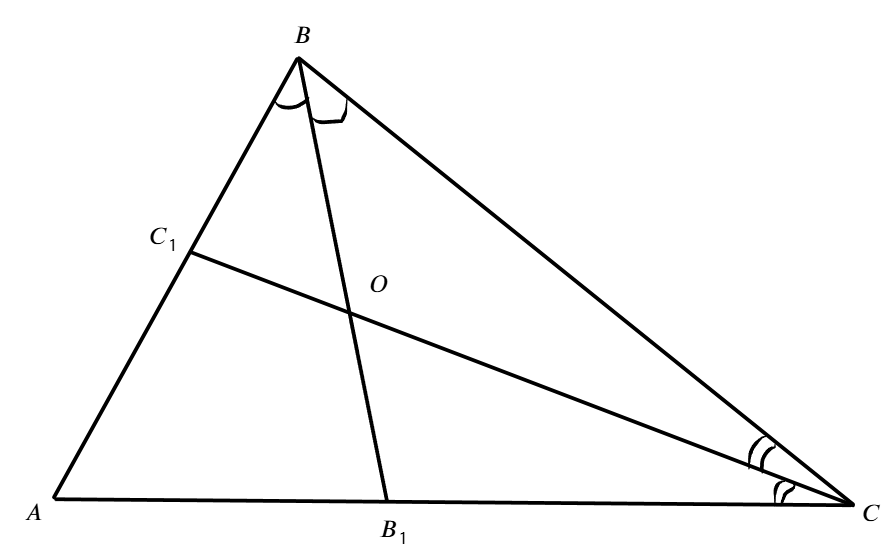
\includegraphics[scale=0.35]{g9-206.png}}
\end{figure}\\
По свойству основания биссектрисы для треугольника $ABC$ имеем соотношение
$\cfrac{AB_1}{CB_1}=\cfrac{AB}{CB}=\cfrac{3}{5},$ при этом $AB_1+CB_1=AC=7,$ откуда $AB_1=\cfrac{3}{8}AC,\ CB_1=\cfrac{5}{8}\cdot7=\cfrac{35}{8}.$ Тогда $\overline{BB}_1=\overline{BA}+\overline{AB}_1=-\vec{b}+\cfrac{3}{8}\vec{c}.$
По свойству основания биссектрисы для треугольника $BB_1C$ имеем соотношение
$\cfrac{BO}{OB_1}=\cfrac{BC}{CB_1}=\cfrac{5}{\cfrac{35}{8}}=\cfrac{8}{7},$ а значит $BO+\cfrac{7}{8}BO=BB_1,\ BO=\cfrac{8}{15}BB_1.$ Таким образом, $\overline{BO}=\cfrac{8}{15}\cdot\left(-\vec{b}+\cfrac{3}{8}\vec{c}
ight)=
\cfrac{1}{5}\vec{c}-\cfrac{8}{15}\vec{b}.$\\
